\documentclass[12pt]{article}
\usepackage[top=1in, bottom=1in, left=1in, right=1in]{geometry}

\usepackage{setspace}
\onehalfspacing

\usepackage{amssymb}
%% The amsthm package provides extended theorem environments
\usepackage{amsthm}
\usepackage{epsfig}
\usepackage{times}
\renewcommand{\ttdefault}{cmtt}
\usepackage{amsmath}
\usepackage{graphicx} % for graphics files

% Draw figures yourself
\usepackage{tikz} 

% writing elements
\usepackage{mhchem}

% The float package HAS to load before hyperref
\usepackage{float} % for psuedocode formatting
\usepackage{xspace}

% from Denovo Methods Manual
\usepackage{mathrsfs}
\usepackage[mathcal]{euscript}
\usepackage{color}
\usepackage{array}

\usepackage[pdftex]{hyperref}
\usepackage[parfill]{parskip}

% math syntax
\newcommand{\nth}{n\ensuremath{^{\text{th}}} }
\newcommand{\ve}[1]{\ensuremath{\mathbf{#1}}}
\newcommand{\Macro}{\ensuremath{\Sigma}}
\newcommand{\rvec}{\ensuremath{\vec{r}}}
\newcommand{\vecr}{\ensuremath{\vec{r}}}
\newcommand{\omvec}{\ensuremath{\hat{\Omega}}}
\newcommand{\sigs}{\ensuremath{\Sigma_s(\rvec,E'\rightarrow E,\omvec'\rightarrow\omvec)}}
\newcommand{\el}{\ensuremath{\ell}}
\newcommand{\sigso}{\ensuremath{\Sigma_{s,0}}}
\newcommand{\sigsi}{\ensuremath{\Sigma_{s,1}}}
%---------------------------------------------------------------------------
%---------------------------------------------------------------------------
\begin{document}
\begin{center}
{\bf NE 250, F15 
}
\end{center}

% 2013-10-01

Recall the one-group diffusion equation:

\begin{equation*}
\frac{1}{v_1}\frac{\partial \phi_1(\rvec,t)}{\partial t} = S_1(\rvec,t) - 
\Sigma_{a,1}(\rvec)\phi_1(\rvec,t) + \nabla\cdot[D_1(\rvec)\nabla\phi_1(\rvec,t)]
\end{equation*}

Now, assume that space and energy dependence of the flux can be separated:

\begin{equation*}
\phi(\vecr,E,t) = \phi(\vecr,t)\psi(E), 
\text{ where $\psi(E)$ is the neutron spectrum and $\int_0^{\infty}dE\psi(E) = 1$.}
\end{equation*}

Focusing on the spatial dependence of the flux, we'll assume a homogeneous steady-state, one-group system.

\begin{equation*}
\frac{1}{v}\frac{\partial\phi(\rvec,t)}{\partial t} = S(\rvec,t) - \Sigma_s(\rvec)\phi(\rvec,t)
+ \nabla\cdot[D(\rvec)\nabla\phi(\rvec,t)]
\end{equation*}

Steady-state: $\frac{1}{v}\frac{\partial\phi(\rvec,t)}{\partial t} = 0$


Homogeneous: no material dependence on position; 
$\Sigma_a(\rvec)\rightarrow\Sigma_a, D(\rvec)\rightarrow D$


This gives us

\begin{equation*}
0 = S(\vecr) - \Sigma_a\phi(\vecr) + D\nabla^2\phi(\vecr)
\end{equation*}

which can be rewritten as

\begin{equation*}
\nabla^2\phi(\vecr) - \frac{1}{L^2}\phi(\rvec) = -\frac{S(\rvec)}{D},
\text{ where $L = \sqrt{\frac{D}{\Sigma_a}} =$ diffusion length.}
\end{equation*}

\begin{equation*}
L = \sqrt{\frac{\langle r^2\rangle}{6}}, \langle r^2\rangle 
=\text{ root mean square distance from birth to absorption}
\end{equation*}

Now, consider a plane source of strength $S_0$ in an infinitely absorbing medium.

\begin{equation*}
\phi(\rvec) = \phi(x)
\end{equation*}

\begin{equation*}
\frac{d^2\phi}{dx^2} - \frac{1}{L^2}\phi(x) = -\frac{S_0\delta(x)}{D}
\end{equation*}

For $x > 0$, $\frac{d^2\phi}{dx^2} - \frac{1}{L^2}\phi(x) = 0$.


Boundary conditions: 
$\lim\limits_{x\rightarrow 0^+}\vec{J}(x) = \frac{S_0}{2}, \lim\limits_{x\rightarrow +\infty}|\phi(x)|<\infty, \phi(x) \geq 0$

For $x > 0$, $\frac{d^2\phi}{dx^2} - \frac{1}{L^2}\phi(x) = 0$.


Boundary conditions: 
$\lim\limits_{x\rightarrow 0^-}\vec{J}(x) = -\frac{S_0}{2}, \lim\limits_{x\rightarrow -\infty}|\phi(x)|<\infty, \phi(x) \geq 0$

With the above equations and boundary conditions, we have a general solution form of

\begin{equation*}
\phi(x) = c_1e^{-x/L} + c_2e^{x/L}.
\end{equation*}

From the finite flux condition, $c_2 = 0$. Then, $\phi(x) = c_1e^{-x/L}$.

\begin{equation*}
\lim\limits_{x\to 0^+} \vec{J}(x) = \lim\limits_{x\to 0^+}\left(\frac{D}{L}c_1e^{-x/L}\right) = 
\frac{D}{L}c_1 = \frac{S_0}{2}
\end{equation*}

\begin{equation*}
c_1 = \frac{S_0 L}{2D}
\end{equation*}

\begin{equation*}
\phi(x) = \frac{S_0L}{2D}e^{-x/L}
\end{equation*}

Now, consider an infinite plane centered in a slab of finite thickness $a$, surrounded by a vacuum.


For $x > 0$, $\frac{d^2\phi}{dx^2} - \frac{1}{L^2}\phi(x) = 0$.


Boundary conditions: 
$\lim\limits_{x\rightarrow 0^+}\vec{J}(x) = \frac{S_0}{2}, \phi(\tfrac{\tilde{a}}{2}) = 0$

For $x < 0$, $\frac{d^2\phi}{dx^2} - \frac{1}{L^2}\phi(x) = 0$.

Boundary conditions: 
$\lim\limits_{x\rightarrow 0^-}\vec{J}(x) = -\frac{S_0}{2}, \phi(-\tfrac{\tilde{a}}{2}) = 0$

\begin{gather*}
\phi(x) = c_1e^{-x/L} + c_2e^{x/L} \\
\text{or} \\
\phi(x) = c_1cosh(\tfrac{x}{L}) + c_2sinh(\tfrac{x}{L})
\end{gather*}

% 2013-10-03

Now, consider a uniformly distributed source of strength $S_0 \tfrac{n}{cm^3s}$ within a finite slab of
width $a$ with vacuum boundaries.

\begin{equation*}
\frac{d^2\phi}{dx^2} - \frac{1}{L^2}\phi(x) = -\frac{S_0}{D}
\end{equation*}

\begin{equation*}
\phi(x) = c_1e^{-x/L} + c_2e^{x/L} + \frac{S_0L^2}{D}
\end{equation*}

Boundary conditions: $\phi(\pm\tfrac{\tilde{a}}{2}) = 0$


Alternative boundary condition: $\frac{d\phi(x)}{dx}\Bigr|_{x = 0} = 0$ (symmetry)


Now, consider a uniform source in a reflected slab like so:

\begin{center}
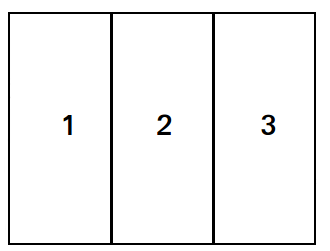
\includegraphics[height=2.5 in]{../figs/ref_slab}
\end{center}

\end{document}
